\documentclass[10pt]{beamer}

%% Use this for 4 on 1 handouts
%\documentclass[handout]{beamer}
%\usepackage{pgfpages}
%\pgfpagesuselayout{4 on 1}[landscape, a4paper, border shrink=5mm]

\usepackage[english]{babel}
\usepackage[utf8]{inputenc}
\usepackage[T1]{fontenc}
\def\subitem{\item[\hspace{1.5cm} -]}

\usepackage{qtree}

% Set the presentation mode to BTH
\mode<presentation>
{
	\usetheme{BTH_msv}
	% Comment this if you do not want to reveal the bullets before they are going to be used
	\setbeamercovered{transparent}
}


% Information for the title page

\title[]{Architectures for Cloud Applications}
\subtitle{}
% \date[]{}

\author[Mikael Svahnberg]{Mikael Svahnberg\inst{1}}
\institute[BTH] % (optional, but mostly needed)
{
  \inst{1}%
 Mikael.Svahnberg@bth.se\\
 School of Computing\\
 Blekinge Institute of Technology%
}

% Delete this, if you do not want the table of contents to pop up at
% the beginning of each subsection:
% \AtBeginSection[]
% {
%  \begin{frame}<beamer>{Outline}
%    \tableofcontents[currentsection,currentsubsection]
%  \end{frame}
% }
\AtBeginSubsection[]
{
 \begin{frame}<beamer>{Outline}
   \tableofcontents[currentsection,currentsubsection]
 \end{frame}
}


% If you wish to uncover everything in a step-wise fashion, uncomment
% the following command: 
%\beamerdefaultoverlayspecification{<+->}

\begin{document}

% Titlepage frame
\begin{frame}
  \titlepage
\end{frame}

% ToC frame
% Use \section and \subsection commands to get things into the ToC.
%\begin{frame}
 %\frametitle{Outline}
 % \tableofcontents
%\end{frame}

% -----------------------------
% Your frames goes here
% -----------------------------
\section{Recap}
\subsection{Software Architectures}

\begin{frame}[t]
\frametitle{Software Architecture Defined}

\begin{itemize}[<+->]
\item First Definition: Boxes and Lines
\begin{itemize}
\item What is the nature of the elements (boxes)?
\item What are the responsibilities of the elements?
\item What is the siginificance of the connections (lines)?
\item What is the significance of the layout?
\end{itemize}
\item Second Definition: Add semantics (provide legend)
\begin{itemize}
\item What is the significance of the layout?
\item What are the interfaces of the elements?
\item How does the architecture operate at runtime?
\item How do we build it?
\end{itemize}
\item Third Definition:\\
\begin{quote}
The software architecture of a program or computing system is the structure or structures of the system, which comprise software elements, the externally visible properties of those elements, and the relationships among them.
\end{quote}
\end{itemize}
\end{frame}


\begin{frame}[t]
\frametitle{Architecture Decisions}

\begin{itemize}
\item Balancing all stakeholders result in a number of \emph{Business and Technical Decisions}
\item Software architecting is about identifying which decisions are necessary, and finding solutions that satisfy all stakeholders.
\end{itemize}

\begin{block}{Decisions \emph{are} the Architecture}
I would go as far as to say that these decisions \emph{are} the architecture.\\
\ldots The rest is just an instantiation of the architecture.
\end{block}
\end{frame}

\begin{frame}[t]
\frametitle{Influences on Architecture}

\begin{itemize}
\item Customer Requirements, of course
\item Developing Organisation
\begin{itemize}
\item e.g., business goals
\item Organisational structure
\item Available expertise (the architect's experience)
\end{itemize}
\item Technical Environment
\end{itemize}
\end{frame}

\begin{frame}[t]
\frametitle{A ``Good'' Software Architecture}

\begin{itemize}
\item Is based on \emph{conscious} decisions
\item Is \emph{evaluated} to ensure that it satisfies the specific goals for the system
\item Pays attention to current and future \emph{quality attributes}
\item Is well \emph{documented}, with traceability to the architecture decisions
\item Features well defined \emph{modules}(components), with well defined \emph{interfaces} and well defined \emph{responsibilities}
\item Is restricted to a small set of interaction patterns that are \emph{consistently} used.
\end{itemize}
\end{frame}


\begin{frame}[t]
\frametitle{Structures and Views}

\begin{columns}%{l}
\column{7cm}%
Bass et al.(2012):

\qtreecenterfalse%
\begin{scriptsize}%
\Tree[.{Module} {Decomposition} {Uses} {Layered} {Class} ]
\vspace{0.5cm}
\Tree[.{Component-and-Connector} {Process} {Concurrency} {Shared Data} {Client-Server} ]
\vspace{0.5cm}
\Tree[.{Allocation} {Deployment} {Implementation} {Work Assignment} ]
\end{scriptsize}%

\column{5cm}%
\only<2->{
Kruchten(1994):

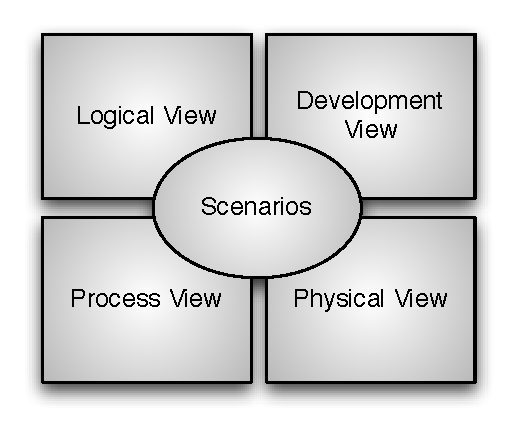
\includegraphics[width=4cm]{FKruchten.pdf}%
}

\only<3->{
Hofmeister et al.(2000) uses a variant of this:
\begin{itemize}
\item Conceptual View
\item Module View
\item Execution View
\item Code View
\end{itemize}
}
\end{columns}
\end{frame}


\begin{frame}[t]
\frametitle{Architecture and Quality Attributes}
\begin{itemize}
\item Functionality is ``easy'' to implement.
\item Quality requirements may \emph{sometimes} have impact on the implementation
\item More often, it impacts the \emph{software structure} (=the software architecture).
\item \ldots And yet, the architecture can only describe a \emph{potential} for achieving a particular quality level.
\end{itemize}
\end{frame}


\subsection{Cloud Relevant Quality Attributes}

\begin{frame}[t]
\frametitle{Factors that ``push'' you towards the cloud}
\begin{itemize}
\item Transference -- Move your on-site solution as-is to the cloud for e.g. economic reasons.
\subitem Challenges: Setting up a similar environment in the cloud as you have locally.
\item Internet Scale -- Scaling up to handle more users.
\subitem Challenges: Database design may become a bottleneck.
\item Burst Compute -- Large swings in capacity requirements.
\subitem Challenges: Strategy for load balancing, database access.
\item Elastic Storage -- Scaling up to handle (much) more data.
\subitem Challenges: need also to consider where the data is processed.
\end{itemize}
\end{frame}


\begin{frame}[t]
\frametitle{Cloud Relevant Quality Attributes}

\begin{itemize}
\item Scalability
\item Reliability / Availability
\item Performance
\item Security
\item Privacy
\item Cost Optimisation
\item Maintainability / Developability
\end{itemize}

\end{frame}

\section{Architecture Implications}
\begin{frame}[t]
\frametitle{Architecture Implications}
\begin{itemize}
\item This is a boring part of the lecture.
\item Basically, we go through each of the cloud relevant quality attributes and discuss the corresponding tactics.
\end{itemize}

\begin{block}{Important}
The most important thing for you to think about, and for us to discuss is:

\vspace{0.5cm}
\emph{How would I address these issues and tactics in my Software Architecture?}
\end{block}

\end{frame}


\subsection{Scalability}
\begin{frame}[t]
\frametitle{Scalability}
\begin{itemize}
\item Horizontal Scaling -- add more nodes
\item Vertical Scaling -- increase capacity of nodes
\item In a Cloud system, you would do both.
\begin{itemize}
\item It is easier to scale vertically unless you already have a horizontally scaled solution
\item Storage space is often easier to deal with by scaling verically -- unless you already have a horizontally scaleable solution in place.
\end{itemize}

\end{itemize}
\end{frame}

\begin{frame}[t]
\frametitle{Scalability Tactics}
Bass et al. does suprisingly not have any tactics associated with Scalability. They list the following tactics for \emph{Performance}:
\begin{itemize}
\item Control Resource Demand
\only<2>{
\begin{itemize}
\item Manage Sampling Rate
\item Limit Event Response
\item Prioritise Events
\item Reduce Overhead
\item Bound Execution Times
\item Increase Resource Efficiency
\end{itemize}
}
\item Manage Resources
\only<3>{
\begin{itemize}
\item Increase Resources
\item Introduce Concurrency
\item Maintain Multiple Copies of Computation
\item Maintain Duplicate Copies of Data
\item Bound Queue Sizes
\item Schedule Resources
\end{itemize}
}
\end{itemize}

\only<4>{
\begin{block}{Discussion}
What else can be done to support scalability \emph{in the application}?
\end{block}
}
\end{frame}

% \begin{frame}[t]
% \frametitle{Architecture Implications of Scalability}
% \begin{itemize}
% \item Load Balancing (Module View/Execution View)
% \item Data Access (Execution View)
% \item Communication and Synchronisation channels (Module View)
% \item Network configuration ((Extended) Execution View)
% \end{itemize}

% But also:
% \begin{itemize}
% \item Cost Optmisation implies that you \emph{first} pursuit solutions such as Docker (Virtual Scaling).
% \subitem This is a good idea for other reasons as well (See Reliability).
% \end{itemize}
% \end{frame}

\subsection{Reliability/Availability}
\begin{frame}[t]
\frametitle{Reliability/Availability}
\begin{itemize}
\item Primary tools: Redundancy, Geographical (and provider) distribution, load balancing.
\item Cloud solutions allows for an informed trade-off between programming reliability in, and throwing redundant servers at the problem.
\item Some Cloud Providers' only availability promise is that \emph{your node will fail after some unspecified time}!
\item Connected to data persistence, since you cannot expect a ``responsible'' node shutdown.
\end{itemize}
\end{frame}


\begin{frame}[t]
\frametitle{Availability Tactics}
Bass et al. list the following Availability Tactics:

\begin{itemize}
\item Detect Faults
\only<2>{
\begin{itemize}
\item Ping/Echo
\item Monitor
\item Heartbeat
\item Timestamp
\item Sanity Checking
\item Condition Monitoring
\item Voting
\item Exception Detection
\item Self-Test
\end{itemize}
}
\item Recover from Faults
\only<3-5>{
\begin{itemize}
\item Preparation and Repair
\only<4>{
\begin{itemize}
\item Active Redundancy
\item Passive Redundancy
\item Spare
\item Exception Handling
\item Rollback
\item Software Upgrade
\item Retry
\item Ignore Faulty Behaviour
\item Degradation
\item Reconfiguration
\end{itemize}
}
\item Reintroduction
\only<5>{
\begin{itemize}
\item Shadow
\item State Resynchronisation
\item Escalating Restart
\item Non-Stop Forwarding
\end{itemize}
}
\end{itemize}
}
\item Prevent Faults
\only<6>{
\begin{itemize}
\item Removal from Service
\item Transactions
\item Predictive Model
\item Exception Prevention
\item Increase Competence Set
\end{itemize}
}
\end{itemize}

\only<7>{
\begin{block}{Discussion}
Which of these would be particularly relevant in a cloud application? Why?
\end{block}
}

\end{frame}

\subsection{Performance}
\begin{frame}[t]
\frametitle{Performance}
\begin{itemize}
\item The way you tackle performance depends very much on what type of performance you are after.
\item For example,
\subitem Response time is very different from
\subitem Processing time, which is very different from
\subitem Storage capacity
\item {[In many applications]} you probably have a mixture of many different requirements.
\end{itemize}
\end{frame}

\begin{frame}[t]
\frametitle{Example: Web application}
\begin{itemize}
\item Response time: System must feel ``snappy''
\item Processing time: Behind the scenes, you may have activities that takes several seconds to perform.
\item For example, submitting a post in a discussion forum may include:
\subitem Re-baking the user's profile
\subitem Looking for cross-posts and re-baking these posts
\subitem Re-generate a thread summary
\subitem \ldots
\item In a sufficiently frequented forum, each of these actions may take several seconds to perform.
\end{itemize}
\end{frame}


\begin{frame}[t]
\frametitle{Example: Cloudbursting}
\begin{itemize}
\item At the other end of the spectrum you have batch-processing applications
\item You use the cloud's computing resouces to (re-) generate massive amounts of data.
\item Response time is not an issue
\end{itemize}
\end{frame}

\begin{frame}[t]
\frametitle{Performance Tactics}
\begin{itemize}
\item Control Resource Demand
\only<2>{
\begin{itemize}
\item Manage Sampling Rate
\item Limit Event Response
\item Prioritize events
\item Reduce Overhead
\item Bound Execution Times
\item Increase Resource Efficiency
\end{itemize}
}
\item Manage Resources
\only<3>{
\begin{itemize}
\item Increase Resources
\item Introduce Concurrency
\item Maintain Multiple Copies of Computations
\item Maintain Multiple Copies of Data
\item Bound Queue Sizes
\item Schedule Resources
\end{itemize}
}
\end{itemize}

\only<4>{
\begin{block}{Discussion}
Which of these would be particularly relevant in a cloud application? Why?
\end{block}
}

\end{frame}


\subsection{Security}
\begin{frame}[t]
\frametitle{Security}
\begin{itemize}
\item Security from External threats
\item Security from threats inside the cloud provider
\begin{itemize}
\item Covert channels between your VM and others'
\item Sniffing network communication
\item Inherently unsafe designs (e.g. Amazon S3's global namespace for their buckets)
\item Legal issues
\end{itemize}

\end{itemize}
\end{frame}


\begin{frame}[t]
\frametitle{Security Tactics}
Bass et al. list the following Security Tactics:
\begin{itemize}
\item Detect Attacks
\only<2>{
\begin{itemize}
\item Detect Intrusion
\item Detect Service Denial
\item Verify Message Integrity
\item Detect Message Delay
\end{itemize}
}
\item Resist Attacks
\only<3>{
\begin{itemize}
\item Identify Actors
\item Authenticate Actors
\item Authorise Actors
\item Limit Access
\item Limit Exposure
\item Encrypt Data
\item Separate Entities
\item Change Default Settings
\end{itemize}
}
\item React to Attacks
\only<4>{
\begin{itemize}
\item Revoke Access
\item Lock Computer
\item Inform Actors
\end{itemize}
}
\item Recover from Attacks
\only<5>{
\begin{itemize}
\item Maintain Audit Trail
\item Restore
\item (See Availability)
\end{itemize}
}
\end{itemize}

\only<6>{
\begin{block}{Discussion}
\begin{itemize}
\item Which tactics can you automate? How?
\item This covers external threats. What about the threats from inside the cloud provider?
\end{itemize}

\end{block}
}

\end{frame}


\subsection{Privacy}
\begin{frame}[t]
\frametitle{Privacy}
\begin{itemize}
\item \emph{Extremely} important
\item The easiest way to get bad publicity is to neglect privacy
\item Often regulated by law.
\item Local laws, that may differ between countries.
\item Ties in with Security: Low security makes it harder to enforce privacy
\end{itemize}
\end{frame}

\begin{frame}[t]
\frametitle{Privacy Tactics}
Not covered by Bass et al. Generic guidelines include:
\begin{itemize}
\item Restrict Stored Personal Information
\subitem What information do you need to store about your users?
\subitem Why?
\subitem For how long?
\item Encrypt Data
\item Use Secure Connections
\item Hire a lawyer!
\subitem Strange as this may seem, this is a cost optimisation. If you do not have to have a replica of your system in each country you cater for just to satisfy local laws, the cost of the lawyer will be recovered quite quickly.
\end{itemize}
\end{frame}

\subsection{Cost Optimisation}
\begin{frame}[t]
\frametitle{Cost Optmisation}
\begin{itemize}
\item The whole purpose of a cloud solution is to optimise CAPEX vs OPEX.
\item The easy solution is to throw more resources at the problem.
\item For obvious reasons, this is not a sustainable solution long-term.
\item \emph{However}, there is a trade-off between how much time your developers should spend on optimising your application and the cost of adding an extra, or a larger cloud resource.
\end{itemize}
\end{frame}

\subsection{Maintainability / Developability}
\begin{frame}[t]
\frametitle{Maintainability / Developability}
\begin{scriptsize}
\begin{itemize}
\item Not a cloud issue \emph{per se}, but becomes more obvious when you are paying for uptime.
\item Each of your developers need a development platform (as usual)
\item Test Environment
\subitem How many test platforms do you need to support? One per developer? One per team?
\subitem How do you provide this? Local Virtual Boxes? On the Cloud?
\item Staging Environment
\subitem As close to your deployment platform as possible
\subitem For extensive ``release-testing''
\subitem How many do you need? Is one enough?
\subitem How do you test the system in the staging environment? Do you need to have a test harness environment too?
\item Deployment Environment
\subitem Do you have just one deployment environment? Or is it one per customer?
\subitem How do you elastically scale this environment? How is this reflected in the staging/testing/development environments?
\end{itemize}
\end{scriptsize}
\end{frame}

\begin{frame}[t]
\frametitle{Supporting different Environments}
\begin{itemize}
\item How do you construct your application such that you can move seamlessly between the different environments?
\item How do you construct your application to support automated builds and tests?
\end{itemize}
\end{frame}

\section{Summary}
\begin{frame}[t]
\frametitle{Summary}
\begin{itemize}
\item Certain Quality Attributes are more relevant than others for a Cloud Application
\item You must first find your particular blend of quality attributes
\item After this, designing a cloud application is similar to designing the architecture for any other system.
\item The Execution View (and hence the Module View) plays a more significant role
\subitem Quite Obviously; this is the factor that has changed.
\item Pay extra attention to \emph{privacy}, and your development environment
\end{itemize}
\end{frame}


% -----------------------------


%% All of the following is optional and typically not needed. 
%\appendix
%\begin{frame}[allowframebreaks]
%  \frametitle{For Further Reading}
%    
%  \begin{thebibliography}{10}
%    
%  \beamertemplatebookbibitems
%  % Start with overview books.

%  \bibitem{Author1990}
%    A.~Author.
%    \newblock {\em Handbook of Everything}.
%    \newblock Some Press, 1990.
%     
%  \beamertemplatearticlebibitems
%  % Followed by interesting articles. Keep the list short. 

%  \bibitem{Someone2000}
%    S.~Someone.
%    \newblock On this and that.
%    \newblock {\em Journal of This and That}, 2(1):50--100,
%    2000.
%  \end{thebibliography}
%\end{frame}

\end{document}


